\pagebreak

\chapter{Code Examples}

    Many of these examples have not been compiled, and those that have
    may not have been executed, hence there may be coding or
    algorithmic errors.

    \section{queue switching}
    
        If we want a pipeline to diverge into one of two or more branches
        we might write a module to do this as follows -
        \begin{lstlisting}[gobble=8, language=threepl]
           module
           diverge (queue({out0, out1}) <- value(select, "log"), queue(in)) {
               when (select)
                   out0 <<- in;
               else
                   out1 <<- in;
           }
        \end{lstlisting}
        This module has two output queues and one input queue. It continuously
        performs one of two assignments depending on the value of logical
        variable {\bf select}. This code however has behaviour that is not
        ideal. If for example queue {\bf in} is not available, execution will
        wait on the selected assignment statement until {\bf in} is available,
        even though {\bf select} might change in the meantime. We could rewrite
        the code as -
        \begin{lstlisting}[gobble=8, language=threepl]
           module
           diverge (queue({out0, out1}) <- value(select, "log"), queue(in)) {
               sync when (select) {
                   out0 <<- in;
               }
               sync when (!select) {
                   out1 <<- in;
               }
           }
        \end{lstlisting}
        Each of the two {\bf sync when} statements will execute on every clock
        cycle. One of these will terminate because the test expression is false
        and the other will either execute the code block because the input and
        output queues are both available or else will also terminate.
        
        Similarly if we wish to converge two queues we could use -
        \begin{lstlisting}[gobble=8, language=threepl]
           module
           converge (queue(out) <- value(select, "log"), queue({in0, in1})) {
               sync when (select) {
                   out <<- in0;
               }
               sync when (!select) {
                   out <<- in1;
               }
           }
        \end{lstlisting}
        Alternatively we could select inputs based on queue availability -
        \begin{lstlisting}[gobble=8, language=threepl]
           module
           converge (queue(out) <- queue({in0, in1})) {
               out <<- in0;        // always when both available
               sync when (!<in0)   // when out and in1 are available but not in0
                   out <<- in1;
           }
        \end{lstlisting}
        (which favours {\bf in0} over {\bf in1}). A {\bf sync when()} will
        only execute the body when all queues in the test expression or
        the body can be read or written (as appropriate) and when the test
        expression is true. When these conditions are not met it does not block!

    \section{a two-cycle module}\label{sec:ex2c}

        This module adds pairs of input data,
        outputing one datum per input pair.
        \begin{lstlisting}[gobble=8, language=threepl]
           queue({q1, q2}, "uint:8");

           .
           .
           [
               static(temp, "uint:8");
               static(second, "log");

               when (second) par {
                   q2 <<- temp + q1;
                   second <- false;
               } else par {
                   temp <- q1;
                   second <- true;
               }
           ]
           .
           .
        \end{lstlisting}
        The {\bf when} will execute repeatedly since it is
        contained immediately within a module, i.e. on
        completion it will begin execution again on the next
        clock cycle. Since the test expression is a static
        variable and thus is always available the {\bf when}
        will pass execution to one of the code bodies
        in the current cycle. Each code body is a parallel
        block. The selected block will execute its enclosed
        statements as soon as possible and will complete
        execution when both have completed. In each block the
        first assignment statement may wait on queue availability
        but the second assignment will execute at once.

        If {\bf second} is false, the second code body will
        begin execution. This is a parallel block so both
        contained statements may execute. The second has no queue
        dependencies so will execute (it toggles the value of
        the test variable). The first has a queue
        dependency so may wait (it saves the datum from the
        input queue). When both have executed, control
        will pass back to the {\bf when} which will complete
        then be executed again.

        If {\bf second} is TRUE, the first code body will begin
        execution. It is similar, but performs the sum and
        writes the result to the output queue. Note that the sum will
        generate a 9-bit result which will be truncated (since it is
        unsigned) on assignment to 8 bits.

        Pairs of input data are summed and the result is the
        output, thus the output queue runs at half the speed of
        the input queue. Logical static variable {\bf second} is
        inverted each time.

        We could force the two assignment statements in each
        block to execute simultaneously by changing the {\bf par}
        blocks to {\bf sync} blocks.
        \begin{lstlisting}[gobble=8, language=threepl]
           queue({q1, q2}, "uint:8");

           .
           .
           [
               static(temp, "uint:8");
               static(second, "log");

               when (second) sync {
                   q2 <<- temp + q1;
                   second <- false;
               } else sync {
                   temp <- q1;
                   second <- true;
               }
           ]
           .
           .
        \end{lstlisting}
        In this case all statements in a block wait until all
        queues referenced anywhere in the block are available at
        which time the statements all execute simultaneously. In
        this example that is not necessary and does not change
        the result. We could also put a {\bf sync} block around the
        {\bf when} instead -
        \begin{lstlisting}[gobble=8, language=threepl]
           queue({q1, q2}, "uint:8");

           .
           .
           [
               static(temp, "uint:8");
               static(second, "log");

               sync{
                   when (second) par {
                       q2 <<- temp + q1;
                       second <- false;
                   } else par {
                       temp <- q1;
                       second <- true;
                   }
               }
           ]
           .
           .
        \end{lstlisting}
        which is subtly different, though it leads to a similar result.
        In this case execution will hang at the {\bf sync} until both queues
        are available at which it will enter the {\bf when} and the true or
        the false block in the {\bf when}, which will execute both statements
        in the {\bf par} simultaneously since we are guaranteed there will be
        no queue waits. This differs slightly from the previous cases if
        {\bf second} is false and {\bf q2} is not available as the {\bf sync}
        will wait for {\bf q2} to become availble, but this is not necessary
        since {\bf q2} is not being written to.

        We could move the assignment of the logical static
        variable {\bf second} out of the {\bf when}, but now must
        enclose the code in a parallel block -
        \begin{lstlisting}[gobble=8, language=threepl]
           queue({q1, q2}, "uint:8");

           .
           .
           [
               static(temp, "uint:8");
               static(second, "log");

               par {
                   when (second)
                       q2 <<- temp + q1;
                   else
                       temp <- q1;
                   second <- !second;
               }
           ]
           .
           .
        \end{lstlisting}
        or could use a {\bf sync} block instead of {\bf par}.
        Without the containing parallel block the two
        components (the {\bf when} and the static assignment)
        would execute independently. Thus logical static
        variable {\bf second} would toggle continuously
        regardless of any queue waits.

        But after all that we could code this example using a sequential
        block! -
        \begin{lstlisting}[gobble=8, language=threepl]
           queue({q1, q2}, "uint:8");

           .
           .
           [
               static(temp, "uint:8");

               seq {
                   temp <- q1;
                   q2 <<- temp + q1;
               }
           ]
           .
           .

        \end{lstlisting}



    \section{loops}
    
        3PL provides target loop control structures, but these are not
        always the best way to implement loops. Take for example a
        module which is to produce a repeating sequence of integers
        from 0 to 9. We might write it as -
        \begin{lstlisting}[gobble=8, language=threepl]
           module
           sequence (queue(out, "uint:4") <- ) {
               static(i, "uint:4");
               
               seq {
                   i <- 0;
                   sync while (i < 10) {
                       out <<- i;
                       i++;
                   }
               }
           }
        \end{lstlisting}
        This code will execute as required, but it wastes one cycle at every
        start of the sequence initialising {\bf i} to 0 and another cycle on the
        final {\bf while} test at which point the loop exits. We could test {\bf
        i} inside the loop and when it reaches 9 reset it to 0, but then we
        would no longer need the {\bf while}. We could instead code the module
        using implicit infinite loops as -
        \begin{lstlisting}[gobble=8, language=threepl]
           module
           sequence (queue(out, "uint:4") <- ) {
               static(i, "uint:4");
               
               sync {
                   out <<- i;
                   when (i == 9)
                       reset(i);   // better than i <- 0
                   else
                       i++;
               }
           }
        \end{lstlisting}
        This generates the sequence with no lost cycles. This
        will enter the {\bf sync} block repeatedly whenever the output
        queue {\bf out} is available. Each time it assigns the next sequence
        value to the output queue and in parallel either increments or zeros
        the index. It will always execute the output queue assignment in one
        cycle because the {\bf sync} has ensured that it is available. Only
        one write to the queue is done and then the {\bf sync} repeats as there
        are no loops within the {\bf sync}.
        
        For nested loops we could again use {\bf while}s -
        \begin{lstlisting}[gobble=8, language=threepl]
           module
           sequence (queue(out, "uint:16") <- ) {
               static(x, "uint:4");
               static(y, "uint:4");
               
               seq {
                   reset(y);
                   seq while (y < 10) {
                       reset(x);
                       sync while (x < 10) {
                           out <<- x | (y << 8);
                           x++;
                       }
                       y++;
                   }
               }
           }
        \end{lstlisting}
        but here we waste more cycles sequentially initialising or
        incrementing loop variables. The above code can probably be
        improved but at the expense of readability. We could again
        change this to use implicit infinite loops -
        \begin{lstlisting}[gobble=8, language=threepl]
           module
           sequence (queue(out, "uint:16") <- ) {
               static(x, "uint:4");
               static(y, "uint:4");
               
               sync {
                   out <<- x | (y << 8);
                   when (x == 9) par {
                       reset(x);
                       when (y == 9)
                           reset(y)
                       else
                           y++;
                   } else
                       x++;
               }
           }
        \end{lstlisting}
        This generates the combined sequence from two nested sequences with no
        lost cycles. This enters the {\bf sync} block repeatedly whenever the
        output queue is available. Each time through it assigns the combined
        sequence value to the output queue and in parallel computes the next {\bf
        x} and {\bf y} values. A disadvantage of this code is that it nests {\bf
        when} statements, which while logically correct can lead to long
        combinatorial logic paths which may not fit within timing constraints.
        The compiler cannot transform this to optimise the code.
        The conditional statements could be separated -
        \begin{lstlisting}[gobble=8, language=threepl]
           module
           sequence (queue(out, "uint:16") <- ) {
               static(x, "uint:4");
               static(y, "uint:4");
               
               sync {
                   out <<- x | (y << 8);
                   when (x == 9) par {
                       reset(x);
                       when (y == 9)
                           reset(y)
                       else
                           y++;
                   } else
                       x++;
                   when (x == 9 && y == 9)
                       reset(y);
                   when (x == 9 && y != 9)
                       y++;
               }
           }
        \end{lstlisting}
        Now we have traded logic depth for logic width but in the process have
        duplicated tests. It is now debatable if this is good or bad as
        duplicated logic can be faster by avoiding fanout routing problems. For
        this reason the compiler does not attempt to eliminate this code
        duplication, leaving it up to the programmer to do so explicitly. If we
        feel we should eliminate duplication we could rewrite the above as -
        \begin{lstlisting}[gobble=8, language=threepl]
           module
           sequence (queue(out, "uint:16") <- ) {
               static({x, y}, "uint:4");
               value(xlimit, "log", x == 9);
               value(ylimit, "log", y == 9);
               
               sync {
                   out <<- x | (y << 8);
                   when (xlimit)
                       reset(x);
                   else
                       x++;
                   when (xlimit && ylimit)
                       reset(y);
                   when (xlimit && !ylimit)
                       y++;
               }
           }
        \end{lstlisting}
        Note that the local variables x, y, xlimit and ylimit could have been
        created inside the sync block, rather than in the scope of the module
        itself, since they are only used within that block.



    \section{a data-dependent module}\label{sec:exddm}

        A module to sum inputs until a zero datum, at which
        point the sum is output.

        \begin{lstlisting}[gobble=8, language=threepl]
           queue(q1, "uint:8");
           queue(q2, "uint:16");

           .
           .
           [
               static(sum, "uint:16");

               when (q1 == 0) sync {
                   q2 <<- sum;
                   sum <- 0;   // could use reset(sum);
               } else
                   sum <- sum + q1;
           ]
           .
           .
        \end{lstlisting}
        Here the {\bf when} test expression will only evaluate when queue {\bf
        q1} is available. If the input queue value is zero, the sum will be
        assigned to the output, otherwise the input will be added to the sum.
        Input queue {\bf q1} was read in the test expression so the datum will
        always be removed. If it was used in the last statement, it will be
        read in the same clock cycle as in the {\bf when} test so this will
        constitute a single read of the queue and the removal of one datum.
        The assignment to queue {\bf q2} may wait on availability. Because of
        this we must delay execution of the entire parallel block until all
        queues are ready (in this case just {\bf q2}) so that the two
        assignments are simultaneous since we are changing {\bf sum} in the
        same parallel block in which we are using its value.

        Multiple simultaneous reads of the same input queue in an execution
        cycle is normal practice. Examines and reads can also be used on a
        queue simultaneously. If one or more reads are executed on an input
        queue in an execution cycle the queue datum will be removed.


    \section{a module with extra cycles}\label{sec:exec}

        Input data are copied to the output, but if the MSB is
        set, a zero is also output. This example
        generates another execution cycle independent
        of input queue availability.

        \begin{lstlisting}[gobble=8, language=threepl]
           queue({q1, q2}, "uint:8");

           .
           .
           [
               static(extra, "log");

               when (extra) par {
                   q2 <<- 0;
                   extra <- false;
               } else sync {
                   q2 <<- q1;
                   when ((q1 & 0x80) != 0)
                       extra <- true;
               }
           ]
           .
           .
        \end{lstlisting}
        The {\bf when} will execute repeatedly inside the implied infinite loop
        (the statement is top-level). The test expression involves no queues so
        will flow on immediately passing execution to one of the code bodies.
        Normally {\bf extra} is false so the second code body will be executed.
        It is a parallel block which will assign the input queue value to the
        output queue. This assignment may wait on either queue. The second
        statement tests the MSB of the input queue value (it may also wait on
        that queue) and if that bit is set, it assigns TRUE to the static
        logical variable {\bf extra}. When both statements have executed the
        parallel block finishes, passing control back to the outer {\bf when}
        which also finishes. The outer {\bf when} now executes again in its
        implied infinite loop, but if {\bf extra} is true it will select the
        first code body. This first parallel block assigns zero to the output
        queue and returns {\bf extra} to false. This code has nested {\bf when}
        statements so would be better coded as -
        \begin{lstlisting}[gobble=8, language=threepl]
           queue({q1, q2}, "uint:8");

           .
           .
           [
               static(extra, "log");

               when (extra) par {
                   q2 <<- 0;
                   extra <- false;
               } else sync {
                   q2 <<- q1;
                   extra <- (q1 & 0x80) != 0;
               }
           ]
           .
           .
        \end{lstlisting}
        Both this code and the one above read queue {\bf q1} in two places.
        Because these take place simultaneously (forced to do so by the
        {\bf sync}) they both pop the same datum.

        We could also code this example using a sequential
        block -
        \begin{lstlisting}[gobble=8, language=threepl]
           queue({q1, q2}, "uint:8");

           .
           .
           [
               sync {
                   seq {   // bad - always takes 2 cycles!
                       q2 <<- ?q1;
                       when ((q1 & 0x80) != 0)
                           q2 <<- 0;
                   }
               }
           ]
           .
           .
        \end{lstlisting}
        The {\bf sync} block is immediately inside the module structure so
        again will execute repetitively. By putting a {\bf sync} around the
        {\bf seq} we have ensured that both queues are available before we
        enter the {\bf seq}. The first sequential statement assigns the value
        of the input queue to the output queue, but examines the input rather
        than reading it. This leaves the datum in place. The second
        sequential statement reads the input queue and if the MSB is set it
        writes a zero to the output queue. However, this code is not good as it
        always takes a minimum of two cycles since the {\bf when} will take
        one cycle even when the test is false.


    \section{interfacing external data}

        The following code illustrates an interface to an external data source.
        The data is clocked but is not present on every clock cycle. A separate
        clock enable input is asserted when data is present on the next clock
        edge.
        \begin{lstlisting}[gobble=8, language=threepl]
             useclock(c100);  // 100MHz default platform clock

             float(dclk_freq, 10.0e6);    // data clock frequency, 10MHz
             clock(dclk_in, frequency=dclk_freq, loc=A_pins[8]);  // data clock input
             clock({dclk, dclk_raw}, frequency=dclk_freq);
             clkdcm(dclk_raw <- dclk_in, clkfb=dclk);     // DCM for data clock
             clockbufg(dclk <- dclk_raw); // data clock   // clock buffer

             queue(d, "uint:8");

             dataInput(d <-);
             process1(...... <- d);
             .
             .
             .

             module
             dataInput (queue(out, "uint:8") <- ) {
                 useclock(dclk);  // use the 10MHz data clock

                 input(data_in, "uint:8", loc=A_pins[0..7]);
                 input(enable_in, "log", loc=A_pins[20]);
                 static(data, "uint:8");
                 static(enable, "log");

                 data <- data_in;
                 enable <- enable_in;

                 when (enable)
                     out <<- data;

                 useclock();         // revert to the default 100MHz clock
             }
        \end{lstlisting}
        The first section interfaces the external 10MHz data clock through a
        DCM and a BUFG. {\bf dclk\_in} is the input from the PAD and associated
        IBUF. This is connected to the input of a DCM. The DCM output is
        {\bf dclk\_raw} which is buffered through a BUFG to get the internal
        distributed data clock {\bf dclk}.
        
        Queue {\bf d} is the data source for further processing. {\bf process1}
        is a module or procedure which contains a pipeline to process the data
        and is not defined here. Queue {\bf d} is asynchronous and is written
        sporadically using the 10MHz {\bf dclk} in module {\bf dataInput()} and
        read using {\bf c100}, the default processing clock.
        
        The module {\bf dataInput} has a single parameter, the output queue {\bf
        out}. This queue delivers valid data from the data input when they
        become available. We assume that the 100MHz pipeline {\bf process1()}
        will keep up with the maximum input data rate of 10MHz.
        
        The module {\bf dataInput} changes the current clock domain to
        {\bf dclk}. The data and enable inputs are synchronous with
        this clock domain and the data is written to queue {\bf out} in this
        clock domain.
        
        The data and enable inputs are clocked on every cycle of {\bf dclk} into
        static variables {\bf data} and {\bf enable}. Now synchronised to {\bf
        dclk} within the FPGA when enable is asserted the data is written to the
        module output queue {\bf out} (whose matching argument is queue {\bf d}
        The current clock domain is then reverted to {\bf c100} on exit from the
        module.
        
        Suppose that we wish to reverse the data bits. There are three ways
        we could do that -
        \blist
        \item   We could simply reverse the order of the data input pins.
        \item   We could just reverse subscripts.
        \item   We could assign the bits from {\bf data} to {\bf out} singly
                (but in parallel of course) in reverse order
        \blend
        
        The first is obvious -
        \begin{lstlisting}[gobble=8, language=threepl]
            input(data_in, "uint:8", loc=A_pins[7..0]);
        \end{lstlisting}
        
        The second can be done by library function {\bf reverse()} -
        \begin{lstlisting}[gobble=8, language=threepl]
            out <<- reverse(data);
        \end{lstlisting}
        
        The third requires casting the data to and from an array -
        \begin{lstlisting}[gobble=8, language=threepl]
            type(t, "[8]bits:1");
            value(v1,, cast(data, t));
            value(v2, t);
            
            for (int(i) ; i<8 ; i++)
                v2[i] := v1[7-i];                    
            out <<- cast(v2, type(out));
        \end{lstlisting}
        
        This could also be done by using library function getbit() -
        \begin{lstlisting}[gobble=8, language=threepl]
            type(t, "[8]bits:1");
            value(v2, t);
            
            for (int(i) ; i<8 ; i++)
                v2[7-i] := getbit(data, i);                    
            out <<- cast(v2, type(out));
        \end{lstlisting}
        
        
        If the enable input is such that it remains asserted for multiple
        clock cycles to delineate a data frame, we may want to include a flag
        on the first datum in each frame.

        \begin{lstlisting}[gobble=8, language=threepl]
            struct (dtype,
                data,   "uint:8",   // data
                first,  "log"       // is this the first frame datum?
            );

            module
            dataInput (queue(out, dtype) <- ) {
                useclock(dclk);  // use the 10MHz data clock

                input(data_in, "uint:8", loc=A_pins[0..7]);
                input(enable_in, "log", loc=A_pins[20]);
                static(data, "uint:8");
                static(enable, "log");

                data <- data_in;
                enable <- enable_in;

                static(first, "log", true);

                when (enable) {
                    out.data <<- data;
                    out.first <<- first;
                    first <- false;
                }
                when (!enable)
                    first <- true;

                useclock();         // revert to the default 100MHz clock
            }
        \end{lstlisting}
        This code is a little slack in that it assumes that the queue {\bf out}
        will always be available for writing. This assumption is reasonable in
        that there is no flow control of the external data source so data would
        be lost if the output of module {\bf dataInput()} did not keep up with
        the data input stream since the write to {\bf out} would hang until it
        became available. Meanwhile the next datum might have overwritten the
        previous. Enclosing the code in a {\bf sync\{\}} would not help as that
        simply moves the write availability check from the individual assignment
        statements to an enclosing block where it would still wait.


    \section{a 1-dimensional pixel window}\label{sec:ex1Dw}

        To create a sliding 3 pixel window from a data
        stream we might consider creating the structure
        shown in \autorefph{fig:ex3wf}.
        \begin{figure}[htbp]
        \centering
        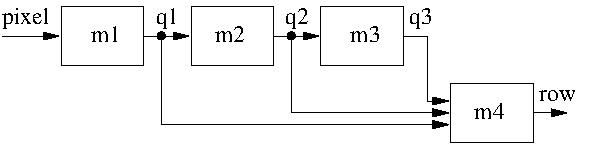
\includegraphics{ex3wf}
        \caption{A 3 pixel window}
        \label{fig:ex3wf}
        \end{figure}
        This is not the best way to implement a window operator.
        
        Firstly module m4 would have to be written so that is first accepted
        q1 only, then q1 with q2 and finally all three queue inputs. If m4
        waits on its 3 inputs it will read the same datum from all 3 and it
        will only output every 3 cycles, the pipeline being delayed 2 cycles
        in every 3. m2 and m3 must hold exactly one datum each, otherwise the
        window will not contain contiguous data. We could get around the
        startup problem by giving queues q2 and p3 initial data.
        
        Secondly these modules as shown would only be unit delays for which
        the queue overheads would be inefficient.
        
        It is far better to implement the window delays as static variables
        within a module.
        \begin{lstlisting}[gobble=8, language=threepl]
           module
           win3 (queue(out, "[3]uint:8") <- queue(in, "uint:8")) {
               static(del, "[2]uint:8");
               
               sync {
                   del[0] <- in;
                   del[1] <- del[0];
                   out[0] <<- in;
                   out[1] <<- del[0];
                   out[2] <<- del[1];
               }
           }        
        \end{lstlisting}
        Note that we needed a {\bf sync} block to bind the execution of the
        queue and static assignments to the availability of queues {\bf in} and
        {\bf out}. With a {\bf par} the two static assignments would have
        executed straight away regardless of the availability of the queues.

        We could parameterise this in a number of ways. Firstly we could make
        the window width a parameter -
        \begin{lstlisting}[gobble=8, language=threepl]
           module
           win1D (queue(out, "["+width+"]uint:8") <- queue(in, "uint:8"), int(width)) {
               static(del, "["+(width-1)+"]uint:8");
               
               sync {
                   del[0] <- in;
                   for (int(i, 1) ; i<(width-1) ; i++)
                       del[i] <- del[i-1];
                   out[0] <<- in;
                   for (int(i, 1) ; i<width ; i++)
                       out[i] <<- del[i-1];
               }
           }        
        \end{lstlisting}
        The above code could be written more simply as -
        \begin{lstlisting}[gobble=8, language=threepl]
           module
           win1D (queue(out, "["+width+"]uint:8") <- queue(in, "uint:8"), int(width)) {
               static(del, "["+(width-1)+"]uint:8");
               
               sync {
                   del[0] <- in;
                   del[1..width-1] <- del[0..width-2];
                   out[0] <<- in;
                   out[1..width-1] <<- del[0..width-2];
               }
           }        
        \end{lstlisting}
        Because input parameters are created and matched with arguments before
        output parameters we can use an immediate input parameter value as a
        dimension for an output parameter. An alternative would have been to
        simply omit any type for the output parameter and let the output
        argument (which must after all be correct) supply the parameter
        dimension.
        \begin{lstlisting}[gobble=8, language=threepl]
           module
           win3 (queue(out) <- queue(in, "uint:8"), int(width)) {
               .
               .
               .
           }        
        \end{lstlisting}
        
        
        We could now make the window module independent of data type, picking
        up the input and output types from the arguments -
        \begin{lstlisting}[gobble=8, language=threepl]
           module
           win1D (queue(out) <- queue(in), int(width)) {
               static(del, "["+(width-1)+"]"+type(in));
               
               sync {
                   del[0] <- in;
                   del[1..width-1] <- del[0..width-2];
                   out[0] <<- in;
                   out[1..width-1] <<- del[0..width-2];
               }
           }        
        \end{lstlisting}
        
        We could simplify this further by making the static the same type as
        the output queue, even though we need an array one smaller -
        \begin{lstlisting}[gobble=8, language=threepl]
           module
           win1D (queue(out) <- queue(in), int(width)) {
               static(del, type(out));
               
               .
               .
               .
           }        
        \end{lstlisting}
        Here we rely on code optimisation to remove the unused array member
        of static variable {\bf del}.
        
        The previous examples do not recognise frame boundaries.
        In practice we might have a frame input signal which is asserted
        during contiguous pixels in a frame and not asserted during frame
        gaps. To carry this signal along with the pixel data a struct would
        be used for the input stream -
        \begin{lstlisting}[gobble=8, language=threepl]
            struct(inpix,
                data,   "uint:8",
                frame,  "log"
            );
        \end{lstlisting}
        where {\bf frame} is true for valid pixels and false for data
        between frames. For the data output there would no longer be a gap
        in the data stream so we could perhaps flag the last window in a frame
        by using another struct -
        \begin{lstlisting}[gobble=8, language=threepl]
            struct(pixwin1,
                data,   "["+winwidth+"]uint:8",
                last,   "log"
            );
        \end{lstlisting}
        We have the choice of filling off-edge pixels in the 3-pixel window with
        a default value (0), adding another field to struct {\bf pixwin1} or
        else restricting the scan width to exclude off-edge pixels. The
        following example takes the second alternative. It is assumed that the
        gap between frames is wider than the window.
                          
        \begin{lstlisting}[gobble=8, language=threepl]
            int(winwidth, 3);
            queue(q1, inpix);
            queue(q2, pixwin1);

            win1D(q2 <- q1, winwidth);
            .
            .
            .

            module
            win1D (queue(out, pixwin1) <- queue(in, inpix), int(width)) {
                if (width%2 == 0)
                    texit("win1D - window width is not odd");
                else
                    int(centre, width / 2);
                static(del, "["+width+"]inpix");

                sync {
                    del[0] <- in;
                    del[1..width-1] <- del[0..width-2];
                    when (del[centre].frame) par {
                        for (int(i) ; i<width ; i++)
                            out.data[i] <<- del[i].data;
                        out.last <<- !del[centre-1].frame;
                    }
                }
            }        
        \end{lstlisting}
        Note that the {\bf sync} requires that both the input and output
        queues be available before the input queue will be read even when
        the window centre is off-edge. This is unlikely to be of concern.


    \section{a 2-dimensional pixel window}\label{sec:ex2Dw}

        We can extend on the previous example to make a 2D window.

        Since we are processing a 2D
        raster we can envisage an input signal that is asserted when a pixel is
        within a line and another that is asserted when a pixel is within a
        frame (frame now has a different meaning to that in the previous
        example). The input pixels will now have two fields in addition to the
        data -
        \begin{lstlisting}[gobble=8, language=threepl]
            struct(inpix,
                data,   "uint:8",   // pixel
                line,  "log",       // pixel within line
                frame,  "log"       // pixel within frame
            );
        \end{lstlisting}
        Here field {\bf line} will be true when a pixel is within a horizontal
        line and field {\bf frame} will be true when a pixel is within a frame.
        During line gaps {\bf line} will be false but {\bf frame} will remain
        true. Thus a pixel is valid when {\bf line} and {\bf frame} are both
        true.
        \begin{lstlisting}[gobble=8, language=threepl]
            struct(inpix,
                data,   "uint:8",   // pixel
                line,   "log",      // pixel within line
                frame,  "log"       // pixel within frame
            );
        \end{lstlisting}
        
        For a 2D array specification we can use a string -
        \begin{lstlisting}[gobble=8, language=threepl]
            int(winwidth, 3);
            str(pixarray, "["+winwidth+"]["+winwidth+"]");
        \end{lstlisting}
        which we can then insert in types -        
        \begin{lstlisting}[gobble=8, language=threepl]
            type(pixwin2D, pixarray+"inpix");
            struct(outpix,
                data,   pixarray+"uint:8",
                lastl,  "log",
                lastf,  "log"
            );
        \end{lstlisting}
        The output struct contains the 2D pixel array {\bf data}, a flag
        indicating that the central pixel is the last pixel in a line {\bf lastl}
        and flag indicating the last line in a frame, {\bf lastf}. {\bf lastf} will
        be true for every pixel window in the last line.



        
        
        \begin{lstlisting}[gobble=8, language=threepl]
            module
            win2D (queue(out, outpix) <- queue(in, inpix), int(linelen)) {
                int(ww, dimension(out.data, 0));    // window width
                if (ww%2 == 0)
                    texit("win2D - window width is not odd");
                else
                    int(centre, ww / 2);            // centre pixel of window
                static(del, pixwin2D);              // window - 2D array of pixels

                sync {
                    del[0][0] <- in;
                    del[1..ww-1][0] <- delay(del[0..ww-2][ww-1], linelen-ww-1,, true);
                    del[0..ww-1][1..ww-1] <- del[0..ww-1][0..ww-2];
                    when (del[centre][centre].line) sync {
                        for (int(i) ; i<ww ; i++)
                            for (int(j) ; j<ww ; j++)
                                out.data[i][j] <<- del[i][j].data;
                        out.lastl <<- !del[centre-1][centre-1].line;
                        out.lastf <<- !del[centre-1][centre-1].frame;
                    }
                }
            }
        \end{lstlisting}
        
        The \verb'..' construction indicates a subscript range. The code above
        connects up the window elements such that each row shifts one left and
        the the input for each row is the leftmost pixel of the previous row
        delayed by the line length - the widow length - 1. If expanded
        explicitly the above would look like -
        \begin{lstlisting}[gobble=8, language=threepl]
            int(ed, linelen-ww-1);  // extra delay - line length - window length - 1

            del[0][0] <- in;                    // input to 1st line

            del[1][0] <- delay(del[0][2], ed);  // 2nd line from end of 1st
            del[2][0] <- delay(del[1][2], ed);  // 3rd line from end of 2nd

            del[0][1] <- del[0][0]; // shift 1st line left
            del[0][2] <- del[0][1]; //   "    "   "    "
            del[1][1] <- del[1][0]; // shift 2nd line left
            del[1][2] <- del[1][1]; //   "    "   "    "
            del[2][1] <- del[2][0]; // shift 3rd line left
            del[2][2] <- del[2][1]; //   "    "   "    "
        \end{lstlisting}
        The library function {\bf delay()} implements a fixed delay. The 1st
        argument is the input. The 2nd argument is the delay line length. The
        3rd argument, if true, specifies that block RAM is to be used to contain
        the data rather than flip-flops or CLB shift registers. This should be
        specified where too many shift registers would be required otherwise.
        
        


    \section{pixel window operations}
    
        To carry out window operations on an image it is necessary to stream the
        image in some useful pixel order. This is not a limitation of 3PL,
        which can access arrays in parallel, but rather a limitation of the
        hardware on which 3PL target code executes. Because of the size of
        image arrays current FPGA-based processing boards can only store
        images in conventional RAM. To access the image it must be read
        through a port, usually one pixel at a time. To create a small window
        which scans through the image the image stream is delayed through
        successive line delay elements and pixel delay elements to form
        a parallel pixel window. Thus an {\bf n x n} window will require
        {\bf n-1} line delays and {\bf n x (n-1)} pixel delays. A pixel delay
        is simply a register but a line delay requires a small FPGA block RAM
        (rmemory). These blocks constitute the main limitation to the number
        and size of window operations we can perform in an FPGA. Of course
        if we can carry out a number of parallel operations on the same
        window we avoid proliferation of these delay elements.

        Using the above pixel window code we can perform the usual image processing
        array operations, for example a Sobel operator could be coded as -
        \begin{lstlisting}[gobble=8, language=threepl]
           int(iwidth, 1024);
           queue({pixel, sob}, "uint:8");
           queue(window, "[3][3]uint:8");
           
           .
           win3x3(window <- pixel, iwidth);
           sobel(sob <- window);
           .
           
           module
           sobel (queue(out) <- queue(in)) {
               value({s1, s2, s3, s4}, "int:10");
               value({m1, m2}, "int:11");
               
               s1 := in[0][0] + 2 * in[1][0] + in[2][0];
               s2 := in[0][2] + 2 * in[1][2] + in[2][2];
               s3 := in[0][0] + 2 * in[0][1] + in[0][2];
               s4 := in[2][0] + 2 * in[2][1] + in[2][2];
               m1 := s2 - s1;
               m2 := s4 - s3;
               out <<- (m1 > 0 ? m1 : -m1) + (m2 > 0 ? m2 : -m2);
           }
        \end{lstlisting}
        Further window operations would require more stages in the pipeline
        of calls to module {\bf pixwin()} and window operator modules.
        
        Note that the above sobel module is correct but it generates large
        combinatorial expressions whose logic depth is likely to prove a problem
        at high clock rates. We could recode it to use internal pipelining
        within the module -
        \begin{lstlisting}[gobble=8, language=threepl]
           module
           sobel (queue(out) <- queue(in)) {
               queue({s1, s2, s3, s4}, "int:10");
               queue({m1, m2}, "int:11");
               
               sync {
                   s1 <<- in[0][0] + 2 * in[1][0] + in[2][0];
                   s2 <<- in[0][2] + 2 * in[1][2] + in[2][2];
                   s3 <<- in[0][0] + 2 * in[0][1] + in[0][2];
                   s4 <<- in[2][0] + 2 * in[2][1] + in[2][2];
               }
               m1 <<- s2 - s1;
               m2 <<- s4 - s3;
               out <<- (m1 > 0 ? m1 : -m1) + (m2 > 0 ? m2 : -m2);
           }
        \end{lstlisting}
        Note that there is a {\bf sync} around the four queue assignment
        statements that read queue {\bf in}. This is not necessary for
        synchronisation since the internal queues {\bf s1} to {\bf s4} can
        only become unavailable simultaneously due to the symmetry of the code
        and hence these four assignments will execute simultaneously as they
        have a common input queue. However, the use of the {\bf sync} means
        that queue availability is only tested once after which the four
        assignments execute without further queue testing. If the {\bf sync}
        were omitted then each assignment would individually test queue
        availability before executing. This would result in duplicated logic,
        but it is not obvious if this would be give larger or smaller
        signal delays (code duplication can give smaller signal delays by
        keeping signal lines short and local).
        


    \section{traversing a memory}\label{sec:traverse}

        The following module traverses a memory from an address supplied
        as an argument (a queue), summing the
        contents until a zero entry is encountered, at which time the sum
        is output. We need to write the code differently depending on whether
        we use combinatorial output memory or registered output memory.
        
        For combinatorial output memory the read occurs within the current
        clock cycle so the data can be used directly. For this reason the
        combinatorial output memory read is a function rather than a
        procedure.
        \begin{lstlisting}[gobble=8, language=threepl]
           cmemory(mem, 1, "uint:8", "uint:8");

           module
           sum (queue(out, "uint:16") <- queue(inaddr, "uint:8")) {
               static(searching, "log");
               static(addr, "uint:8");
               static(sum, "uint:16");
               value(mrv, "uint:8", cmemoryread(mem, 0, addr));

               when (searching)
                   when ((mrv == 0)) sync {
                       reset(searching, sum);
                       out <<- sum;
                   } else par {
                       sum <- sum + mrv;
                       addr++;
                   }
               else sync {
                   sum <- cmemoryread(mem, 0, inaddr);
                   addr <- inaddr + 1;
                   searching <- true;
               }
           }
        \end{lstlisting}
        Initially {\bf searching} is false (by default) so the {\bf else} of the
        outer {\bf when} will be executed. This is a {\bf sync} which will wait
        for the starting address queue {\bf inaddr} to be available. When {\bf
        inaddr} is available the memory location whose address in {\bf in} will
        be read and assigned to the sum {\bf sum} and logical static {\bf
        searching} will be assigned {\bf true}. The search address {\bf addr}
        will be assigned {\bf in + 1} ready to continue the scan.
        
        The {\bf sync} starting the outer {\bf else} block is not strictly
        necessary as there is only one queue to be waited on and both dependent
        statements will hence execute at the same time. Also it does not matter
        if the assignment to {\bf searching} occurs in a separate clock cycle to
        the queue reads. The use of {\bf sync} there however will save checking
        the availability of {\bf inaddr} on two deparate statements.
        
        Note that for combinatorial output memory the output always reflects the
        current address input so despite the function name there is no explicit
        read.

        The outer {\bf when} will repeat in its implied infinite loop and this
        time will execute the true body. We want to do the memory read and then
        decide what action to take. By assigning the memory read function to a
        value variable, {\bf mrv} (memory read value), we can use the result in
        two places, the inner {\bf when} test expression and then optionally
        adding the value to the sum. It is important that the memory read and
        the address increment occur in the same clock cycle in the {\bf par}
        block, but there is no problem there as no queues are involved so there
        will be no queue waits.
        
        When {\bf searching} is true and {\bf mrv} is zero the sum can be
        written to queue {\bf out}. Since {\bf sum} is zeroed (along with searching)
        in the same parallel block as it is written to queue {\bf out} the block
        must be a {\bf sync} otherwise the sum will be zeroed whie waiting for
        the output queue to be available should it not already be so.    

        Note that the memory scan proceeds even if the output queue is not
        available right up until it is time to write the result to the output
        queue at which point there might be a wait on output queue availability.
        
        The nested when statements in the code above could be eliminated
        by detecting the three distinct states -
        \begin{lstlisting}[gobble=8, language=threepl]
           cmemory(mem, 1, "uint:8", "uint:8");

           module
           sum (queue(out, "uint:8") <- queue(inaddr, "uint:8")) {
               static(searching, "log");
               static(addr, "uint:8");
               static(sum, "uint:16");
               value(mrv, "uint:8", cmemoryread(mem, 0, addr));
               value(ieq0, "log", mrv == 0);

               sync {
                   when (searching && ieq0) sync {
                       reset(searching, sum);
                       out <<- sum;
                   }
                   when (searching && !ieq0) par {
                       sum <- sum + mrv;
                       addr++;
                   }
                   when (!searching) sync {
                       sum <- cmemoryread(mem, 0, inaddr);
                       addr <- in + 1;
                       searching <- true;
                   }
               }
           }
        \end{lstlisting}
        The sync will execute in an implied infinite loop as usual. The three
        {\bf when} statements will execute simultaneously within the {\bf sync}
        but the conditional expressions are mutually exclusive so that only one
        of them will execute its code block. The surrounding {\bf sync} locks
        them together, otherwise if one were waiting on a queue wait another may
        find that its conditional expression has changed and then it might begin
        execution at the same time. The {\bf sync} ensures that only one can execute
        at a time, given that their conditional expressions are mutually
        exclusive at the time of entry to the {\bf sync}. We could also
        achieve the same by using individual {\bf sync} statements -
        \begin{lstlisting}[gobble=8, language=threepl]
           cmemory(mem, 1, "uint:8", "uint:8");

           module
           sum (queue(out, "uint:8") <- queue(inaddr, "uint:8")) {
               static(searching, "log");
               static(addr, "uint:8");
               static(sum, "uint:16");
               value(mrv, "uint:8", cmemoryread(mem, 0, addr));
               value(ieq0, "log", mrv == 0);

               when (searching && ieq0) sync {
                   reset(searching);
                   out <<- sum;
               }
               when (searching && !ieq0) sync {
                   sum <- sum + mrv;
                   addr++;
               }
               when (!searching) sync {
                   sum <- cmemoryread(mem, 0, inaddr);
                   addr <- inaddr + 1;
                   searching <- true;
               }
           }
        \end{lstlisting}

        For registered output memory the output becomes available in the cycle
        following a read, the read being explicit.
        \begin{lstlisting}[gobble=8, language=threepl]
           rmemory(mem, 1, "uint:8", "uint:8");

           module
           sum (queue(out, "uint:8") <- queue(inaddr, "uint:8")) {
               static(searching, "log");
               static(addr, "uint:8");
               static(sum, "uint:16");
               value(mrv, "uint:8", rmemoryout(mem, 0));
               value(ieq0, "log", mrv == 0);

               when (searching && ieq0) sync {
                   reset(searching);
                   out <<- sum;
               }
               when (searching && !ieq0) sync {
                   sum <- sum + mrv;
                   rmemoryread(mem, 0, addr);
                   addr++;
               }
               when (!searching) sync {
                   rmemoryread(mem, 0, inaddr);
                   reset(sum);
                   addr <- inaddr + 1;
                   searching <- true;
               }
           }
        \end{lstlisting}
        This executes much as the previous example but will execute one extra
        memory read, which will not be used. The variable {\bf mrv} now
        represents the value of the memory output register holding the result of
        a memory read on a previous cycle.
        
        On the first memory read the result is not available until the next
        clock cycle. On the following clock cycle the previous read result
        is added to {\bf sum}, another memeory read is executed and the address
        is incremented, all in parallel.
        
        We could code the solution differently as follows
        \begin{lstlisting}[gobble=8, language=threepl]
           rmemory(mem, 1, "uint:8", "uint:8");

           module
           sum (queue(out, "uint:8") <- queue(inaddr, "uint:8")) {
               static(addr, "uint:8");
               static(sum, "uint:16");
               value(mrv, "uint:8", rmemoryout(mem, 0));

               seq {
                   sync {
                       rmemoryread(mem, 0, inaddr);
                       addr <- inaddr + 1;
                       sum <- 0;
                   }
                   while (mrv != 0) par {
                       rmemoryread(mem, 0, addr);
                       sum <- sum + mrv;
                       addr++;
                   }
                   out <<- sum;
               }
           }
        \end{lstlisting}
        This is an endlessly repeating sequence of three
        parts. The first reads the memory location given by the
        input queue {\bf inaddr}. This will wait until the input queue
        is available. Following this a {\bf while} loop continues
        until it encounters a zero entry, summing the values
        as it goes. The final part writes out the sum to the
        output queue (possibly waiting on its availability).
        This solution is more readable.
        
        The three examples above might be shortened by overlapping
        the output assignment with the next address input.



    \section{searching a linked list in memory}\label{sec:link}

        This illustrates linked list traversal using static
        variables. The memory contains items structured as link
        plus data. The queue function is passed an initial
        memory address. It follows links in the memory until it
        finds a zero address. At that point it outputs the
        associated data item.
        \begin{lstlisting}[gobble=8, language=threepl]
           str(type, "uint:8");
           struct(item,
               data,  type,
               addr,  type
           );
           rmemory(mem, 1, type, item);
           
           module
           find (queue(out, type) <- queue(inaddr, type)) {
               static(searching, "log");
               value(mrv, item, rmemoryout(mem, 0));

               if (!searching) par {
                   rmemoryread(mem, 0, inaddr);
                   searching <- true;
               } else par {
                   if (mrv.addr == 0) par {
                       reset(searching);
                       out <<- mrv.data;
                   } else
                       rmemoryread(mem, 0, mrv.addr);
               }
           }
        \end{lstlisting}

        As in the previous section we could write instead -
        \begin{lstlisting}[gobble=8, language=threepl]
           str(type, "uint:8");
           struct(item,
               data,  type,
               addr,  type
           );
           rmemory(mem, 1, type, item);

           module
           find (queue(out, type) <- queue(in, type)) {
               static(i, item);

               seq {
                   rmemoryread(mem, 0, in);
                   while (i.addr != 0)
                       rmemoryread(mem, 0, i.addr);
                   out <<- i.data;
               }
           }
        \end{lstlisting}



    \section{function generation using look-up tables}\label{sec:fglut}

        Arbitrary function generation can be performed by means of a
        look-up table. For example to generate a stream of sin values
        to a queue -
        \begin{lstlisting}[gobble=8, language=threepl]
            var(mi, "[256]uint");
            for (int(i) ; i<256 ; i++)
                mi[i] = 2048 + floor(2047.0 * sin(2 * i * math_pi / 256.0));

            rmemory(m, 1, "uint:8", "uint:12", mi);

            static(addr, "uint:8");
            queue(sinstream, "uint:12", depth=16);

            sync {
                rmemoryread(m, 0, addr);
                sinstream <<- rmemoryout(m, 0);
                addr++;
            }
        \end{lstlisting}
        The sin values are generated by immediate code and used as an
        initialisation array for the block RAM (rmemory). The 12 bit values are
        offset by 2048 so that they are positive. The rmemory has an 8 bit
        address to hold 256 values and the stored values are 12 bit unsigned.

        The following code takes the sin stream and drives an external MCP4822
        DAC to produce an analog sin wave. The data stream to the DAC is much
        slower than the sin generation which just waits, generating values when
        the queue {\bf sinstream} is not full.
        
        \begin{lstlisting}[gobble=8, language=threepl]
            module "spi.3pl"

            useclock(c32);  // 32MHz clock domain

            // sin generation code inserted here

            static({_cs, _ldac}, "log", true);
            static({sdi, sck}, "log");
            struct(s,
                val,        "uint:12",
                active,     "log",
                gain_low,   "log",
                dummy,      "log",
                select,     "uint:1"
            );
            queue(data, s);

            output(,, _cs, loc=C_pins[0]);  // DAC chip select
            output(,, sdi, loc=C_pins[1]);  // DAC serial data in
            output(,, sck, loc=C_pins[2]);  // DAC serial clock
            output(,, _ldac, loc=C_pins[3]);// DAC load value

            seq {
                sync {
                    data.select <<- 0;  // select A output
                    data.gain_low <<- true; // X1 gain
                    data.active <<- true;   // active
                    data.val <<- sinstream; // DAC value
                }
                _ldac <- false;
                _ldac <- true;
                wait(781.241e-6);       // delay for 5Hz 256 sample/cycle sin
            }

            value(spi_step, "log");     // SPI serial transmission step - 4MHz 32 / 8)
            seq {
                assert(spi_step <- );   // 1 cycle
                nop(7);                 // wait 7 cycles
            }

            spi_master(sck, sdi, _cs <- data,, spi_step);
        \end{lstlisting}
        
        This can be expanded to multi-phase by interleaved reads of the sin
        table since the table reads are very much faster in this case than
        the data transmitted to the DAC. Multiple DACs can be driven in parallel.









    \section{signal processing}\label{sec:dsp}
    
        It is not usually appropriate to use queue mode variables for
        signal processing pipelines. Queue mode variables are queues
        whereas what is required is a chain of registers. In a processing
        pipeline where queue mode variables are used each datum moves along
        the pipeline at clock rate regardless of other data. If input
        data is unavailable the pipeline empties from the input end.
        If the output is blocked then data fill the pipeline and become
        queued. A signal processing pipeline is implemented using a chain
        of registers where data is available on every clock cycle and the
        output is never blocked. Each register in the pipeline contains one
        datum. The data move in lock step every clock cycle.

        A signal processing schematic is shown in
        \autorefph{fig:dspex1}.
        \begin{figure}[htbp]
        \centering
        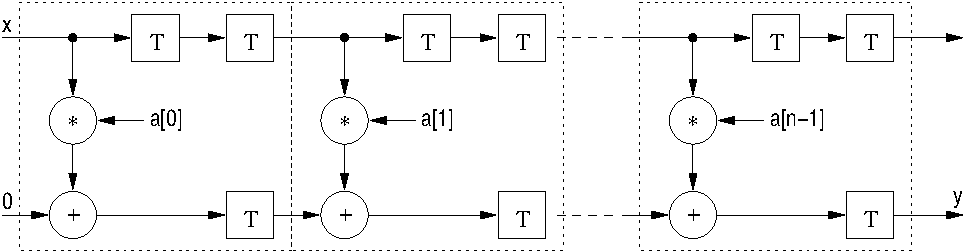
\includegraphics{dspex1}
        \caption{Simple signal processing example}
        \label{fig:dspex1}
        \end{figure}

        The code for a single stage might be -
        \begin{lstlisting}[gobble=8, language=threepl]
           module
           section (
               static({out0, out1}, "fixed:12.6")
               <-
               value({in0, in1}, "fixed:12.6"), float(a)
           ) {
               static(s, "fixed:12.6");
               
               s <- in0;
               out0 <- s;
               out1 <- a * in0 + in1;
           }
        \end{lstlisting}
        For simplicity and generality the input and output parameter types can
        be omitted, in which case the types of the arguments will be used -
        \begin{lstlisting}[gobble=8, language=threepl]
           module
           section (static({out0, out1}) <- value({in0, in1}), float(a)) {
               static(s, type(in0));
               
               s <- in0;
               out0 <- s;
               out1 <- a * in0 + in1;
           }
        \end{lstlisting}
        
        The complete filter could be constructed by -
        
        \begin{lstlisting}[gobble=8, language=threepl]
           int(n, 50);
           var(x_pins, "["+n+"]string", {"A2", "B4", ......}); // FPGA input pins
           var(y_pins, "["+n+"]string", {.........});          // FPGA output pins
           var(a, "["+n+"]float", {3.1, 2.7, ..........});     // coefficients
           input(x, "fixed:12.6", loc=x_pins);
           value(v1, "fixed:12.6", i1);
           value(v2, "fixed:12.6", 0);
           
           for (int(i) ; i<n ; i++) {
               section(v1, v2 <- v1, v2, a[i]);
           }
           
           output(,, v2, loc=y_pins);
        \end{lstlisting}
        Note the use of value variables {\bf v1} and {\bf v2} as both input
        and output arguments to the module {\bf section}. On each call the
        prior value of each variable is used and on each return these
        variables point to the new output parameter static variables. Thus
        {\bf v1} and {\bf v2} act as links between successive calls to construct the
        processing pipeline chain.

        A less regular example is shown in
        \autorefph{fig:dspex2}.
        \begin{figure}[htbp]
        \centering
        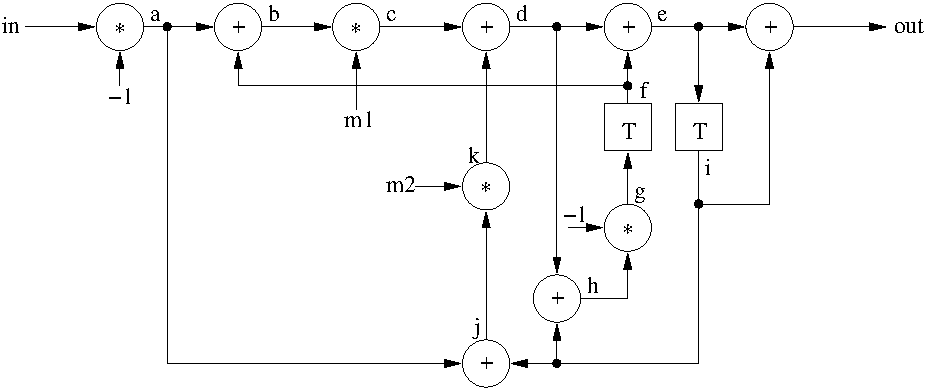
\includegraphics{dspex2}
        \caption{Complicated signal processing example}
        \label{fig:dspex2}
        \end{figure}
        This example is an IIR, or recursive, filter from
        a text on digital filters. The
        code for this is -
        \begin{lstlisting}[gobble=8, language=threepl]
           module filter (queue(in, "uint:16") <- queue(out, "uint:16")) {
               static({f, i}, "uint:16");
               value({a, b, c, d, e, g, h, j, k}, "uint:16");
               int(m1, ...);
               int(m2, ...);

               sync {
                   f <- g;
                   i <- e;

                   a := -in;
                   b := a + f;
                   c := b * m1;
                   d := c + k;
                   e := d + f;
                   g := -h;
                   h := i + d;
                   j := a + i;
                   k := j * m2;

                   out <<- e + i;
               }
           }
        \end{lstlisting}
        This could be shortened to -
        \begin{lstlisting}[gobble=8, language=threepl]
           module filter (queue(in, "uint:16") <- queue(out, "uint:16")) {
               static({f, i}, "uint:16");
               value({d, e, g}, "uint:16");
               int(m1, ...);
               int(m2, ...);

               sync {
                   f <- g;
                   i <- e;

                   d := (f - in) * m1 + (i - in) * m2;
                   e := d + f;
                   g := d - i;

                   out <<- e + i;
               }
           }
        \end{lstlisting}


    \section{A batcher parallel sorting network}\label{sec:batcher}

        A batcher sort network is generated by an
        algorithm, which must be written as immediate code. The following
        module creates a batcher sorting network for any number of inputs
        greater than 2. The input and output queues must be arrays of the same
        size and type {\bf uint} or {\bf int}.
        \begin{lstlisting}[gobble=8, language=threepl]
           module
           sort (queue(out) <- queue(in)) {
               int(inputs, dimension(in));
               int(stages, get_stages(inputs));
               int(sbits);     // bits to hold 'size'
               int(size2);     // power of 2 containing window size
               int(i);
               int({p, q, r}); // Batcher parameters
               int(d); // Batcher parameter - distance between exchange pairs
               int(wi);        // window member index
               int(si);        // network stage index
               var(ignore, "["+inputs+"]log"); // flags for skipping 2nd of exchange pair
               var(net, "["+(stages+1)+"]->");
               net[0] = &in;
               queuearray(net[1..stages-1] <- type(in));
               net[stages] = &out;

               for (i=inputs-1 ; i!=0 ; i=i>>1)
                   sbits++;
               size2 = 1 << (sbits - 1);

               for (p=size2 ; p>0 ; p=p>>1) {
                   r = 0;
                   d = p;
                   for (q=size2 ; q!=(p/2) ; q=q>>1) {
                       [
                           for (wi=0 ; wi<inputs ; wi++)
                               if (ignore[wi])        // already connected
                                   ignore[wi] = false;
                               else if ((wi < (inputs-d)) && ((wi & p) == r)) {// exchange
                                   cond_exchange ( net[si+1]->[wi], net[si+1]->[wi+d]
                                                   <-
                                                   net[si]->[wi], net[si]->[wi+d] );
                                   ignore[wi+d] = true;// ignore later
                               } else                  // straight through
                                   net[si+1]->[wi] <<- net[si]->[wi];
                       ]
                       d = q - p;
                       r = p;
                       si++;
                   }
               }
           }
        \end{lstlisting}
        Notice that the input and output queues are the only arguments passed
        to the module, all necessary parameters being derived from the
        characteristics of the input queue. The intermediate {\bf for} loop
        with loop variable {\bf q} generates an inline module on each
        iteration, each module handling one parallel stage of the sort. The
        stages are pipelined together. The inner loop generates conditional
        exchange assignments or direct assignments.
        
        The code needs an array of queues for the multi-stage network and since
        we cannot implement that directly a pointer array is used. The first
        and last pointers in the array are to the input and output queues. The
        intermediate pointers are to queues created by the library procedure
        {\bf queuearray()}.
        
        The immediate code which generates the target code uses
        Batcher's algorithm which will not be described here. The number of
        stages needed for the sort is determined by the following immediate
        function -
        \begin{lstlisting}[gobble=8, language=threepl]
           function
           get_stages (int(size)) {
               int({sbits, stages});

               for (int(i, size-1) ; i!=0 ; i=i>>1)
                   sbits++;
               for (stages=0 ; sbits>0 ; sbits--)
                   stages = stages + sbits;
               return(stages);
           }
        \end{lstlisting}
        Conditional exchanges are implemented by the following procedure -
        \begin{lstlisting}[gobble=8, language=threepl]
           procedure
           cond_exchange (queue(o0), queue(o1) <- queue(i0),  queue(i1)) {
               value(gt01, "log");

               gt01 := i0 > i1;
               par {
                   o0 <<- gt01 ? i1 : i0;
                   o1 <<- gt01 ? i0 : i1;
               }
           }
        \end{lstlisting}
